\chapter{Result and Evaluation of Simulations}\label{chap:results}
In the following the simulations are presented for the different topologies. The networksizes chosen for the simulations are to the base 2. For an overview of the conducted simulations, one can refer to table \ref{table:overviewsims}. We also conducted simulations to the base 10, which one can find in the \hyperref[chap:appendix]{Appendix}.
The graph is a so-called \textit{log-log graph}, meaning that we have logarithmic scales for both, the x-axis showing the number of rounds and the y-axis representing the scale for the mean squared error. The Single-Proposal-Deal-Agreement-Based algorithm is abbreviated in the following as \textit{DAB}, while the Push-Pull Sum algorithm is abbreviated as \textit{PPS}. In each subsection a winner is singled-out. The Simulations

\section{Complete Graphs}
\textbf{The Complete graph}: The complete graph as depicted in \hyperref[fig:completegraphDemo]{figure} \ref{fig:completegraphDemo} is a graph where each pair of distinct nodes is connected by an edge. The complete graph contains of $n$ nodes and $\frac{n\times(n-1)}{2}$ edges. Every node has a degree of $n-1$, since each node is connected to every other node except to itself \cite{GraphTheorySchindelhaauer2021}. The complete graph is a dense graph, since it has the maximal amount of edges for a given number of nodes.
\begin{figure}
    \centering
    \input{figures/completeGraphSimulations/completegraph.tex}
    \caption{Complete graph: network size 16}
    \label{fig:completegraphDemo}
\end{figure}
\subsection{Network Size 2\textsuperscript{4}}
\textbf{Analysis}: The plot of figure \ref{fig:16CompleteGraph} indicates that the MSE of the network balanced by the DAB algorithm does not initially fall as significantly compared to the PPS. In round 29, the MSE suddenly manages to reduce the error of the network to 0. An MSE of 0 suggests a balanced network. All nodes have the same load. This is exactly the state we are aiming for. Despite the initially steeper downward slope of the PPS graph, the DAB ultimately manages to balance the graph more quickly. The remaining simulation showed that in some cases the DAB protocol reduces the error of the network faster, however there are cases like in the \hyperref[chap:appendix]{Appendix} where the PPS performs better for small network sizes. \\
The number of edges for a network size of 16 is 120. The PPS chooses its load transfer by random. For the PPS each load transfer step involves a push and a pull operation. For a small network size the PPS cannot already exploit the high connectivity of the graph. With increasing network change the PPS will perform better as we see. On the other hand, it is possible for the DAB algorithm to fully balance the network within 50 rounds, since each load transfer involves the maximal possible fair load. \\
\textbf{Winner}: DAB/PPS\\
\begin{figure}[H]
    \centering
    \includegraphics[scale=0.5]{figures/completeGraphSimulations/DAB_vs_PPS_FCG_r50_n16.png}
    \caption{Fully connected graph: network size $2^{4}$ nodes}
    \label{fig:16CompleteGraph}
\end{figure}

\subsection{Network Sizes 2\textsuperscript{8}, 2\textsuperscript{12}, 2\textsuperscript{14}}
\textbf{Analysis}: For bigger network sizes PPS outperforms DAB. The plots of figures \ref{fig:256CompleteGraph}, \ref{fig:4096CompleteGraph} and \ref{fig:16384CompleteGraph} indicate this very clearly. The plots show that DAB maintains a consistent MSE of the network of around 1,000 across all rounds, indicating that it does not improve (or change) significantly over time. PPS, on the other hand reaches a significant decrease in MSE as the number of rounds increases, indicating that PPS improves a lot better than DAB with more rounds and achieves a much lower error, reaching down to less than $1e-14$.\\
\textbf{Winner}: PPS
\begin{figure}[H]
    \centering
    \includegraphics[scale=0.5]{figures/completeGraphSimulations/DAB_vs_PPS_FCG_r50_n256.png}
    \caption{Fully connected graph: network size $2^{8}$ nodes}
    \label{fig:256CompleteGraph}
\end{figure}

\begin{figure}[H]
    \centering
    \includegraphics[scale=0.5]{figures/completeGraphSimulations/DAB_vs_PPS_FCG_r50_n4096.png}
    \caption{Fully connected graph: network size $2^{12}$ nodes}
    \label{fig:4096CompleteGraph}
\end{figure}
\begin{figure}[H]
    \centering
    \includegraphics[scale=0.5]{figures/completeGraphSimulations/DAB_vs_PPS_FCG_r50_n16384.png}
    \caption{Fully connected graph: network size $2^{14}$ nodes}
    \label{fig:16384CompleteGraph}
\end{figure}


\section{Star Graph}
\textbf{The star graph}: A star graph as depicted in \hyperref[fig:stargraphDemo]{figure} \ref{fig:stargraphDemo} is a complete bipartite graph \cite{west2001introduction}. A graph is characterized as bipartite graph, if the set of graph edges is the union of two disjoint independent sets \cite{GraphTheorySchindelhaauer2021}. The central node is part of one set, while the remaining outer nodes are part of another set. A star with $n$ nodes has $n-1$ edges. The degree of every node is 1, except for one node, which has the degree of $n-1$. The diameter of a star graph is 2.
\begin{figure}
    \centering
    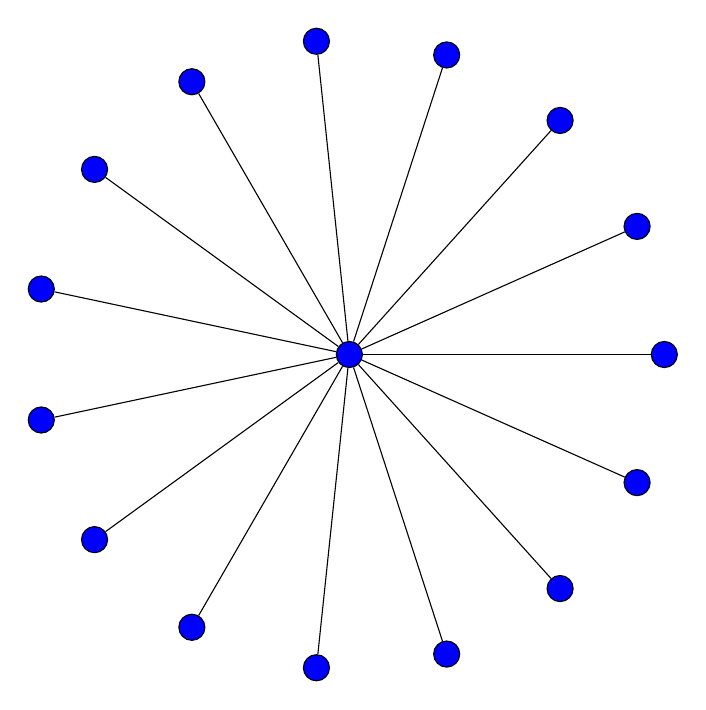
\begin{tikzpicture}
    \node[draw, fill=blue, circle] (center) at (0, 0) {};
    \foreach \i in {1,...,15} {
            \node[draw, fill=blue, circle] (n\i) at ({360/15 * (\i-1)}:4) {};
            \draw (center) -- (n\i);
        }
\end{tikzpicture}
    \caption{Star graph: network size 16}
    \label{fig:stargraphDemo}
\end{figure}
\subsection{Network Sizes 2\textsuperscript{4}, 2\textsuperscript{8}, 2\textsuperscript{12}, 2\textsuperscript{14}}
\textbf{Analysis}: The PPS algorithm outperforms the DAB in terms of error reducing in every network size we have simulated. For small network sizes, you can at least see a drop in the curve. In the end, however, the network balanced with the DAB algorithm still has an MSE of around 0.001. The network balanced with the PPS algorithm has already reached an MSE of $1e-23$ and is therefore far more balanced. For larger network sizes, there is no longer a straight line for the DAB balanced network. Instead, a stagnating graph can be observed. A look at the simulation outputs shows: For the three network sizes $2^{8}$, $2^{12}$ and $2^{14}$, the MSE in the 50th round for the DAB balanced network is around 100. meanwhile, the MSE of the PPS balanced network is $<1e-20$, and therefore far better. This is due to the characteristic structure of the star graph. The star graph is a complete bipartite graph, with only the central node in one set and all other nodes in the other set. Each outer node is only connected to the inner node. For the DAB, this means that when searching for the minimum node, only the inner node comes into question. However, if the inner node has a higher load than the outer node, a load transfer is already ruled out. This behaviour means that the network error is reduced very slowly. The PPS, on the other hand, benefits from such a structure. Each node selects the inner node as a trading partner. This means that every node is also involved in a load transfer per round. Each push action of the outer node is followed by a pull action of the inner node. What is now observable, however, is that the inner node is involved in all load transfers. This node therefore fulfils a large part of the balancing procedure. This can lead to problems to the extent that a load transfer is not exactly a cheap operation. If a node is involved in every load transfer, this means a very one-sided load on a node. For the DAB in the star graph scenario there is also a one-sided loading of a node, however with much less load transfers per round. Another observation that emerges from the graph is that the PPS algorithm does not have the ‘anytime’ property. In rounds 47-50, there is a short-term increase in the error for the three network sizes $2^{8}$, $2^{12}$ and $2^{14}$. Such behaviour is not observed for the DAB algorithm.\\
\textbf{Winner}: PPS
\begin{figure}[H]
    \centering
    \includegraphics[scale=0.5]{figures/starGraphSimulations/DAB_vs_PPS_SG_r50_n16.png}
    \caption{Star graph: network size $2^{4}$ nodes}
    \label{fig:16StarGraph}
\end{figure}

\begin{figure}[H]
    \centering
    \includegraphics[scale=0.5]{figures/starGraphSimulations/DAB_vs_PPS_SG_r50_n256.png}
    \caption{Star graph: network size $2^{8}$ nodes}
    \label{fig:256StarGraph}
\end{figure}

\begin{figure}[H]
    \centering
    \includegraphics[scale=0.5]{figures/starGraphSimulations/DAB_vs_PPS_SG_r50_n4096.png}
    \caption{Star graph: network size $2^{12}$ nodes}
    \label{fig:4096StarGraph}
\end{figure}

\begin{figure}[H]
    \centering
    \includegraphics[scale=0.5]{figures/starGraphSimulations/DAB_vs_PPS_SG_r50_n16384.png}
    \caption{Star graph: network size $2^{14}$ nodes}
    \label{fig:16384StarGraph}
\end{figure}

\section{Closed Chain Graph}
\textbf{The closed chain graph}: A closed chain graph (or also refered to as closed path graph) is a regular graph where each node has a degree of two. A chain graph can be drawn so that all of its vertices and edges lie on a single straight line \cite{gross1998graph}. For a closed chain graph, the first and the last node are also connected as depicted in \hyperref[fig:closedChainGraphDemo]{figure } \ref{fig:closedChainGraphDemo}. Furthermore, a closed chain graph has $n$ edges.
\begin{figure}
    \centering
    \scalebox{0.8}{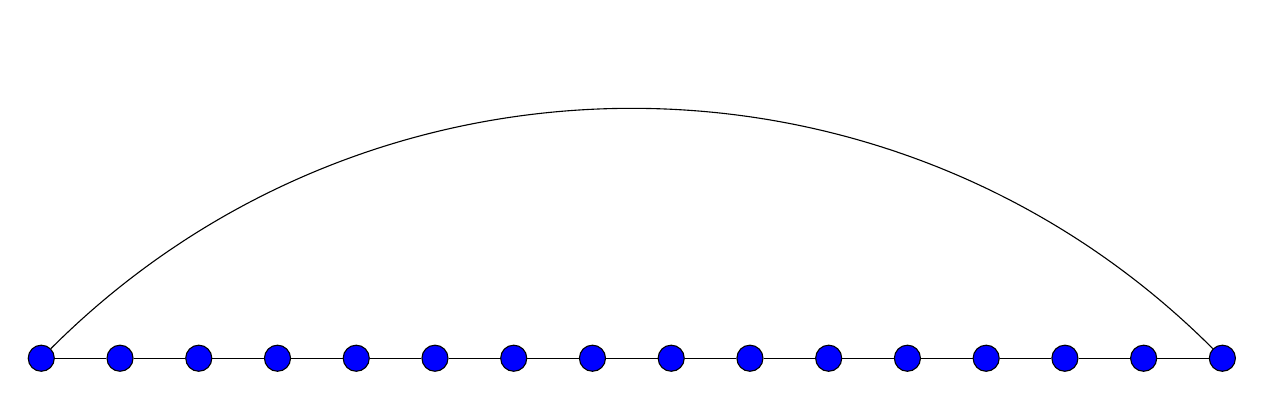
\begin{tikzpicture}
    \foreach \i in {1,...,16} {
      \node[draw, fill=blue, circle, minimum size=6pt] (v\i) at (\i, 0) {};
    }
    
    \foreach \i in {1,...,15} {
      \pgfmathtruncatemacro{\j}{\i+1}
      \draw (v\i) -- (v\j);
    }
    
    \draw[bend left=45] (v1) to (v16);
  
  \end{tikzpicture}}
    \caption{Closed chain graph: network size 16}
    \label{fig:closedChainGraphDemo}
\end{figure}
\subsection{Network sizes 2\textsuperscript{4}, 2\textsuperscript{8}, 2\textsuperscript{12} and 2\textsuperscript{14}}
\textbf{Analysis}:  \\
\textbf{Winner}: DAB\\
\begin{figure}[H]
    \centering
    \includegraphics[scale=0.5]{figures/closedChainSimulations/DAB_vs_PPS_CCG_r50_n16.png}
    \caption{Closed chain graph: network size $2^{4}$ nodes}
    \label{fig:16ChainGraph}
\end{figure}

\begin{figure}[H]
    \centering
    \includegraphics[scale=0.5]{figures/closedChainSimulations/DAB_vs_PPS_CCG_r50_n256.png}
    \caption{Closed chain graph: network size $2^{8}$ nodes}
    \label{fig:256ChainGraph}
\end{figure}

\begin{figure}[H]
    \centering
    \includegraphics[scale=0.5]{figures/closedChainSimulations/DAB_vs_PPS_CCG_r50_n4096.png}
    \caption{Closed chain graph: network size $2^{12}$ nodes}
    \label{fig:4096ChainGraph}
\end{figure}

\begin{figure}[H]
    \centering
    \includegraphics[scale=0.5]{figures/closedChainSimulations/DAB_vs_PPS_CCG_r50_n16384.png}
    \caption{Closed chain graph: network size $2^{14}$ nodes}
    \label{fig:16384ChainGraph}
\end{figure}

\section{Torus Grid Graph}
\begin{figure}
    \centering
    \scalebox{1.5}{\input{figures/torusGridGraphSimulations/torus.tex}}
    \caption{Torus grid graph: network size 16}
    \label{fig:torusGraphDemo}
\end{figure}
\textbf{The torus grid graph}: \cite{PasdeloupTranslationOnGraphs2017}.
\section{Ring of Cliques}
\textbf{The ring of cliques}: \cite{Mahlmann2010}
\begin{figure}
    \centering
    \scalebox{1}{\input{figures/ringOfCliquesSimulations/ringofcliques.tex}}
    \caption{Ring of cliques: network size 16}
    \label{fig:ringofcliquesDemo}
\end{figure}

\section{Lollipop Graph}
\textbf{The lollipop graph}: \cite{JonassonLollipopGraphs2000}
\begin{figure}
    \centering
    \scalebox{1}{\input{figures/lollipopGraphSimulations/lollipopgraph.tex}}
    \caption{Lollipop graph: network size 16}
    \label{fig:lollipopgraphDemo}
\end{figure}